% vim: set spell spelllang=en tw=100 et sw=4 sts=4 foldmethod=marker foldmarker={{{,}}} :

\documentclass[aspectratio=169,compress,10pt]{beamer}

\usepackage{tikz}
\usepackage{xcolor}
\usepackage{complexity}
\usepackage{hyperref}
\usepackage{microtype}
\usepackage{amsmath}                   % \operatorname
\usepackage{amsfonts}                  % \mathcal
\usepackage{amssymb}                   % \nexists
\usepackage[vlined]{algorithm2e} % algorithms
\usepackage{centernot}
\usepackage{mathtools}
\usepackage{listings}
\usepackage{pifont}
\usepackage{bussproofs}
\usepackage{marvosym}

\usefonttheme{professionalfonts}

\usetikzlibrary{shapes, arrows, shadows, calc, positioning, fit}
\usetikzlibrary{decorations.pathreplacing, decorations.pathmorphing, shapes.misc}
\usetikzlibrary{tikzmark, backgrounds}
\usetikzlibrary{trees}
\usetikzlibrary{overlay-beamer-styles}

\definecolor{uofguniversityblue}{rgb}{0, 0.219608, 0.396078}

\definecolor{uofgheather}{rgb}{0.356863, 0.32549, 0.490196}
\definecolor{uofgaquamarine}{rgb}{0.603922, 0.72549, 0.678431}
\definecolor{uofgslate}{rgb}{0.309804, 0.34902, 0.380392}
\definecolor{uofgrose}{rgb}{0.823529, 0.470588, 0.709804}
\definecolor{uofgmocha}{rgb}{0.709804, 0.564706, 0.47451}
\definecolor{uofgsandstone}{rgb}{0.321569, 0.278431, 0.231373}
\definecolor{uofgforest}{rgb}{0, 0.2, 0.129412}
\definecolor{uofglawn}{rgb}{0.517647, 0.741176, 0}
\definecolor{uofgcobalt}{rgb}{0, 0.615686, 0.92549}
\definecolor{uofgturquoise}{rgb}{0, 0.709804, 0.819608}
\definecolor{uofgsunshine}{rgb}{1.0, 0.862745, 0.211765}
\definecolor{uofgpumpkin}{rgb}{1.0, 0.72549, 0.282353}
\definecolor{uofgthistle}{rgb}{0.584314, 0.070588, 0.447059}
\definecolor{uofgrust}{rgb}{0.603922, 0.227451, 0.023529}
\definecolor{uofgburgundy}{rgb}{0.490196, 0.133333, 0.223529}
\definecolor{uofgpillarbox}{rgb}{0.701961, 0.047059, 0}
\definecolor{uofglavendar}{rgb}{0.356863, 0.301961, 0.580392}

\tikzset{vertex/.style={draw, circle, inner sep=0pt, minimum size=0.5cm, font=\small\bfseries}}
\tikzset{notvertex/.style={vertex, color=white, text=black}}
\tikzset{plainvertex/.style={vertex}}
\tikzset{vertexc1/.style={vertex, fill=uofgburgundy, text=white}}
\tikzset{vertexc2/.style={vertex, fill=uofgsandstone, text=white}}
\tikzset{vertexc3/.style={vertex, fill=uofgforest, text=white}}
\tikzset{vertexc4/.style={vertex, fill=uofgheather, text=white}}
\tikzset{edge/.style={color=black!50!white}}
\tikzset{bedge/.style={ultra thick}}
\tikzset{edged/.style={color=screengrey, dashed}}
\tikzset{edgel3/.style={color=uofgrose, ultra thick}}

% {{{ theme things
\useoutertheme[footline=authortitle]{miniframes}
\useinnertheme{rectangles}

\setbeamerfont{block title}{size={}}
\setbeamerfont{title}{size=\large,series=\bfseries}
\setbeamerfont{section title}{size=\large,series=\mdseries}
\setbeamerfont{author}{size=\normalsize,series=\mdseries}
\setbeamercolor*{structure}{fg=uofguniversityblue}
\setbeamercolor*{palette primary}{use=structure,fg=black,bg=white}
\setbeamercolor*{palette secondary}{use=structure,fg=white,bg=uofgcobalt}
\setbeamercolor*{palette tertiary}{use=structure,fg=white,bg=uofguniversityblue}
\setbeamercolor*{palette quaternary}{fg=white,bg=black}
\setbeamercolor{block body}{bg=structure!10}
\setbeamercolor{block title}{bg=structure,fg=white}
\setbeamertemplate{blocks}[rounded]
\setbeamercolor*{titlelike}{parent=palette primary}

\beamertemplatenavigationsymbolsempty

\setbeamertemplate{title page}
{
    \begin{tikzpicture}[remember picture, overlay]
        \node at (current page.north west) {
            \begin{tikzpicture}[remember picture, overlay]
                \fill [fill=uofguniversityblue, anchor=north west] (0, 0) rectangle (\paperwidth, -2.6cm);
            \end{tikzpicture}
        };

        \node (logo) [anchor=north east, shift={(-0.8cm,-0.2cm)}] at (current page.north east) {
            
\includegraphics[keepaspectratio=true,scale=0.5]{UoG_keyline.pdf}
        };

        \node (logo2) [anchor=north, below=0.2cm of logo.south] {
            
\includegraphics[keepaspectratio=true,scale=0.1]{RAEngWhite.pdf}
        };

        \coordinate (logos) at ($(logo.south)!0.5!(logo2.north)$);

        \node [anchor=west, xshift=0.8cm] at (current page.west |- logos) {
            \begin{minipage}{0.65\paperwidth}\raggedright
                {\usebeamerfont{title}\usebeamercolor[white]{}\inserttitle}\\[0.1cm]
                {\usebeamerfont{author}\usebeamercolor[white]{}\insertauthor}
            \end{minipage}
        };
    \end{tikzpicture}
}

\setbeamertemplate{section page}
{
    \begin{centering}
        \begin{beamercolorbox}[sep=12pt,center]{part title}
            \usebeamerfont{section title}\insertsection\par
        \end{beamercolorbox}
    \end{centering}
}

\newcommand{\frameofframes}{/}
\newcommand{\setframeofframes}[1]{\renewcommand{\frameofframes}{#1}}

\makeatletter
\setbeamertemplate{footline}
{%
    \begin{beamercolorbox}[colsep=1.5pt]{upper separation line foot}
    \end{beamercolorbox}
    \begin{beamercolorbox}[ht=2.5ex,dp=1.125ex,%
        leftskip=.3cm,rightskip=.3cm plus1fil]{author in head/foot}%
        \leavevmode{\usebeamerfont{author in head/foot}\insertshortauthor}%
        \hfill%
        {\usebeamerfont{institute in head/foot}\usebeamercolor[fg]{institute in head/foot}\insertshortinstitute}%
    \end{beamercolorbox}%
    \begin{beamercolorbox}[ht=2.5ex,dp=1.125ex,%
        leftskip=.3cm,rightskip=.3cm plus1fil]{title in head/foot}%
        {\usebeamerfont{title in head/foot}\insertshorttitle}%
        \hfill%
        {\usebeamerfont{frame number}\usebeamercolor[fg]{frame number}\insertframenumber~\frameofframes~\inserttotalframenumber}
    \end{beamercolorbox}%
    \begin{beamercolorbox}[colsep=1.5pt]{lower separation line foot}
    \end{beamercolorbox}
}

\makeatletter
\setbeamertemplate{mini frame}
{%
  \begin{pgfpicture}{0pt}{0pt}{.04cm}{.04cm}
    \pgfpathcircle{\pgfpoint{0.04cm}{0.04cm}}{0.04cm}
    \pgfusepath{fill,stroke}
  \end{pgfpicture}%
}
\setbeamertemplate{mini frame in current subsection}
{%
  \begin{pgfpicture}{0pt}{0pt}{.04cm}{.04cm}
    \pgfpathcircle{\pgfpoint{0.04cm}{0.04cm}}{0.04cm}
    \pgfsetfillcolor{section in head/foot.bg}
    \pgfusepath{fill,stroke}
  \end{pgfpicture}%
}

\setbeamersize{mini frame size=0.10cm, mini frame offset=0.06cm}
\makeatother

% }}}

\author{Ciaran McCreesh}
\title{Parallel Constraint Programming}

\begin{document}

{
    \usebackgroundtemplate{
        \tikz[overlay, remember picture]
        \node[at=(current page.south), anchor=south, inner sep=0pt]{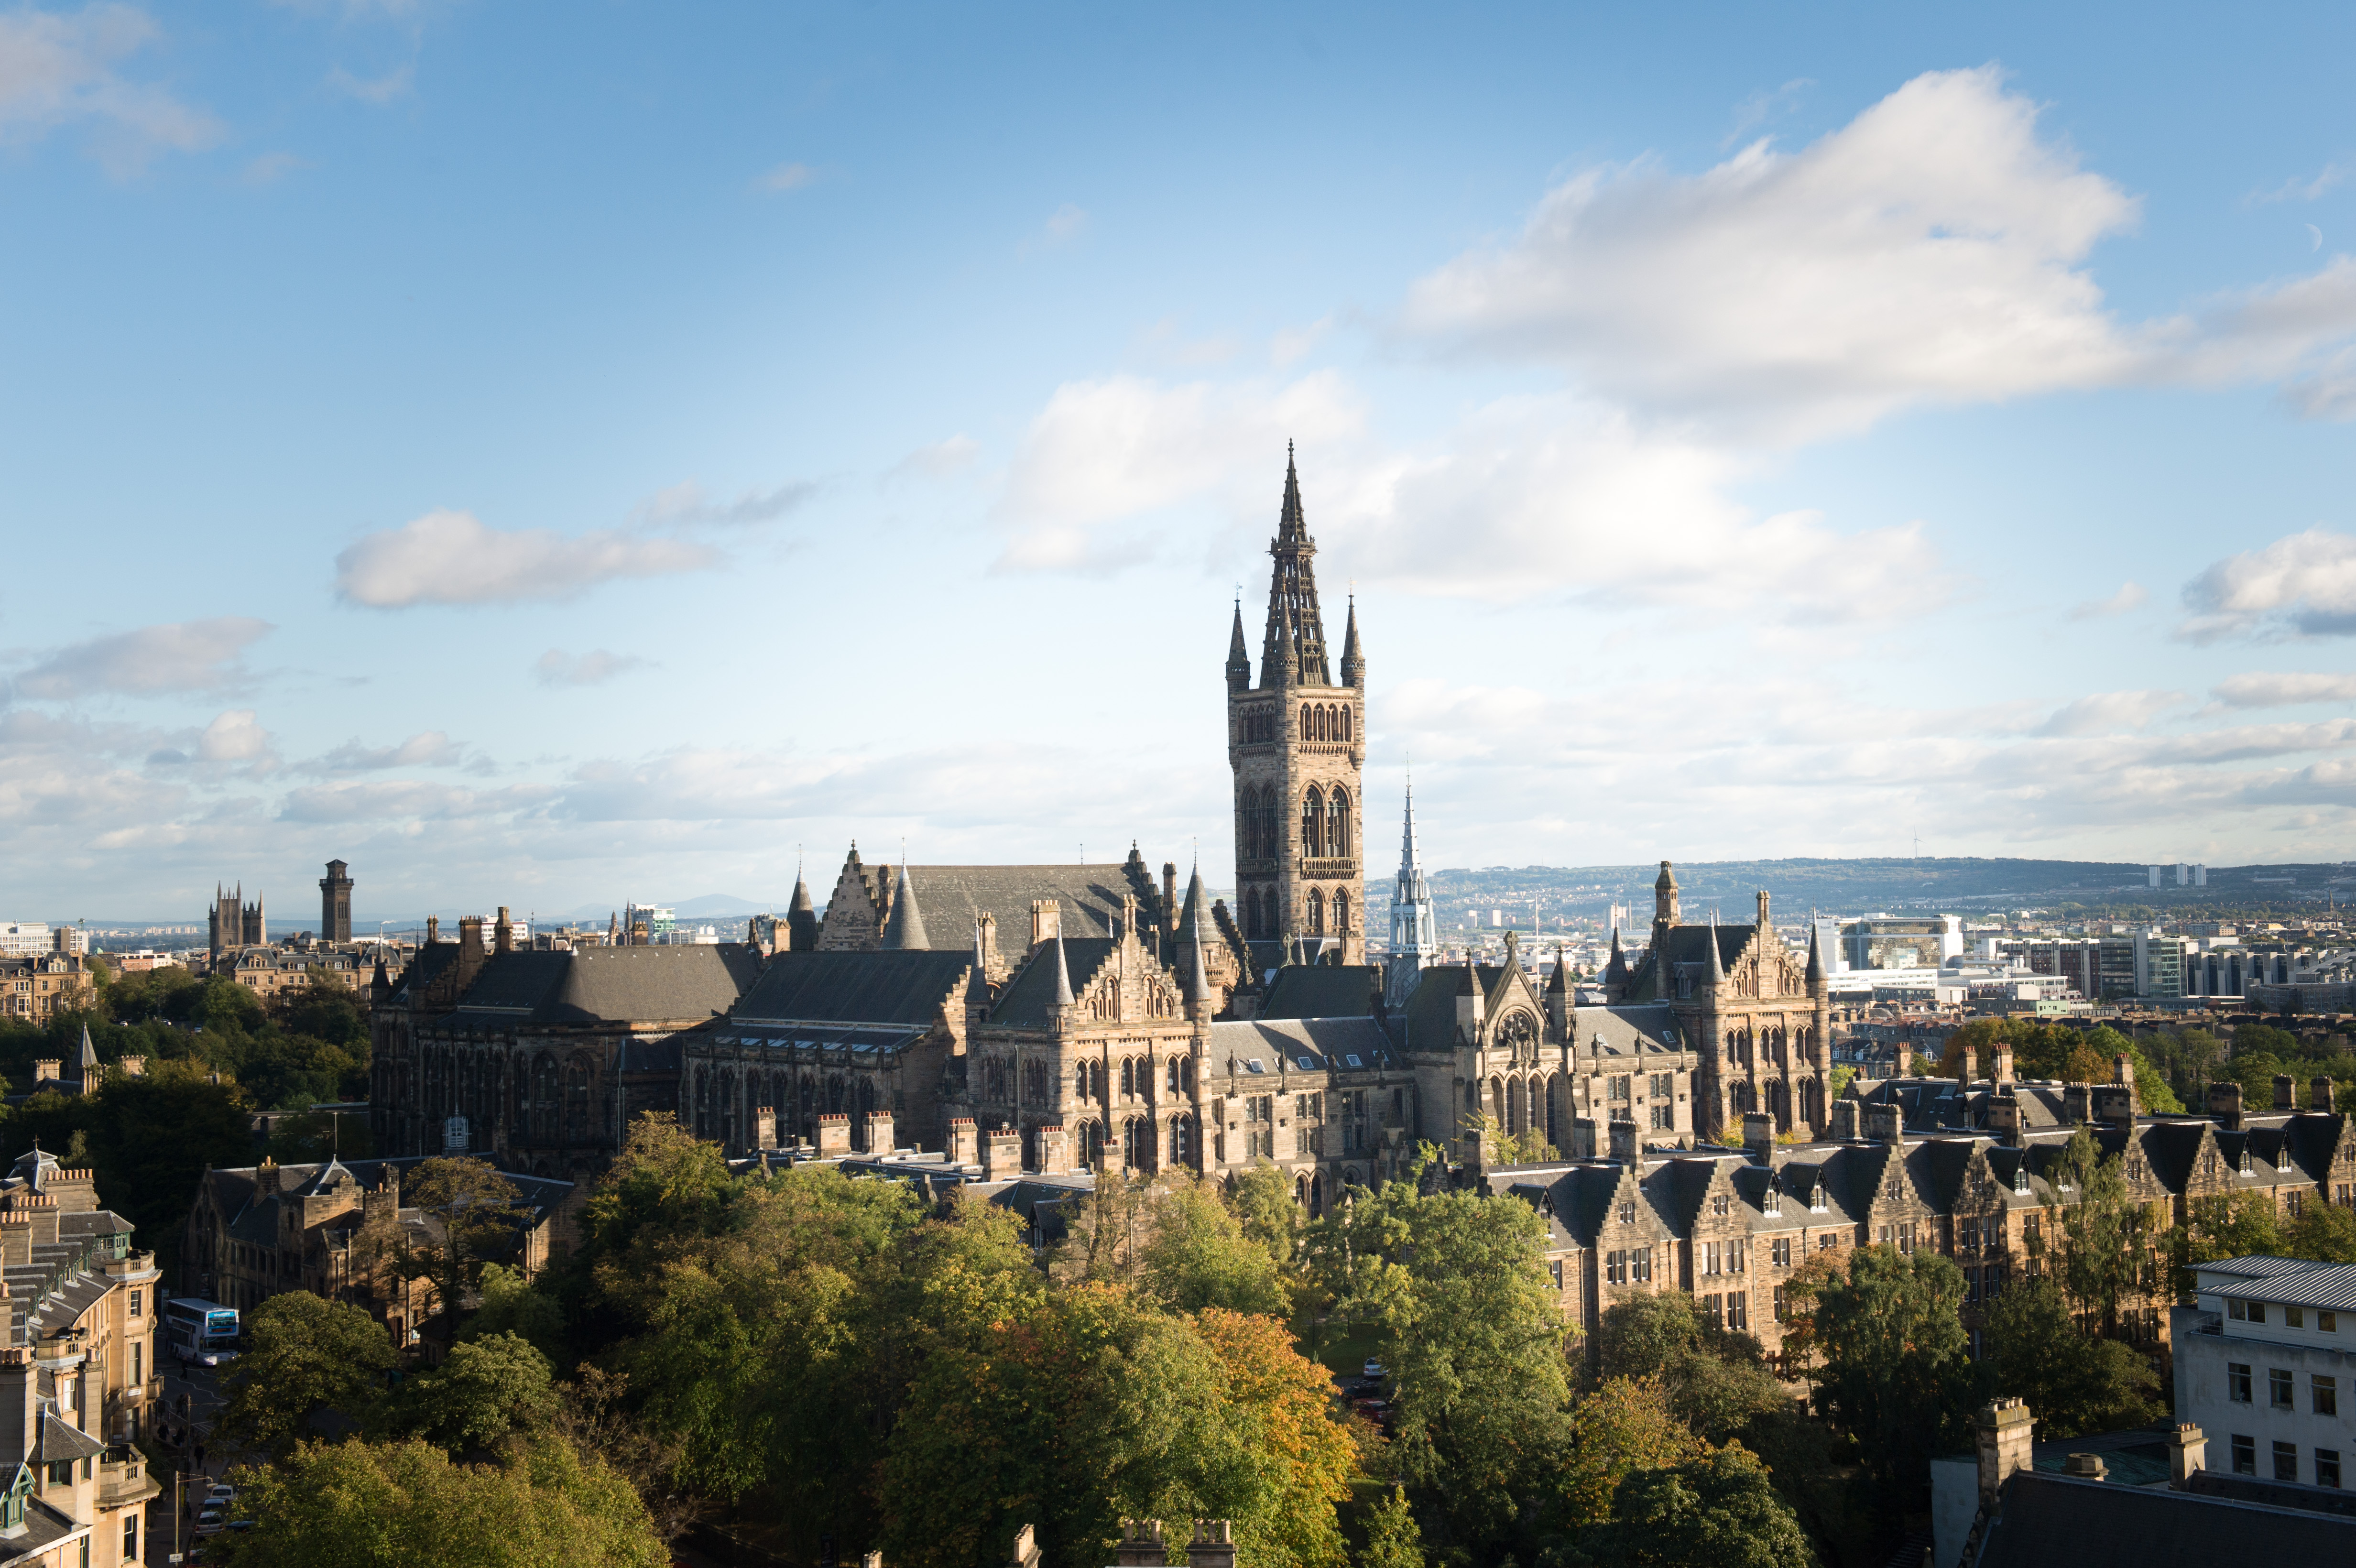
\includegraphics[keepaspectratio=true, width=\paperwidth]{background5.jpg}};
    }
    \begin{frame}[plain,noframenumbering]
        \titlepage
    \end{frame}
}

\begin{frame}[t]{Motivation}
    \begin{itemize}
        \item My laptop when I wrote these slides in 2019: 4 cores.
        \item Current research group compute cluster: 32 cores per machine.
        \item <2-> This laptop: 12 cores.
        \item <2-> Newly purchased compute cluster: 96 cores per machine.
    \end{itemize}

    \vfill
    \centering \includegraphics<1>[keepaspectratio=true,scale=0.08]{fatanode.png}
    \centering \includegraphics<2>[keepaspectratio=true,scale=0.15]{fatanode2.png}
\end{frame}

\begin{frame}{Parallelism and Concurrency}
    \begin{itemize}
        \item Concurrent: lots of stuff happening at once (GUIs, operating systems, networking).

        \item Parallel: our hardware can do more than one thing at once (multi-core, multi-machine,
            vector processing, GPUs).
    \end{itemize}
\end{frame}

\begin{frame}{Goals}
    \begin{enumerate}
        \item Make slow things run faster.
            \begin{itemize}
                \item If ``today's list of parcels to be delivered'' isn't available until 5am, and
                    producing ``today's delivery schedule'' takes twelve hours, we're in trouble. If
                    it takes one hour, we're OK.

                \item If it takes one second, we don't care if we can reduce it to one tenth of a
                    second. (Or maybe we do. What if we're producing results interactively?)
            \end{itemize}

        \item Deal with bigger or harder problems in ``the amount of time we have''.
            \begin{itemize}
                \item We have a fixed amount of time (say, a week) to produce exam timetables. If
                    the University offers more courses, or more flexibility in course choices, we
                    need to solve a larger and harder problem in the same amount of time.
            \end{itemize}
    \end{enumerate}
\end{frame}

\begin{frame}{Unfortunately\ldots}
    \begin{itemize}
        \item Parallel constraint programming is hard.
        \item Most of this lecture is about techniques that don't usually work very well in
            practice. The goal is to understand \emph{why} these techniques fail.
        \item We'll eventually see some techniques that usually work fairly well, most of the time,
            if you don't investigate too closely.
    \end{itemize}
\end{frame}

\begin{frame}[fragile]{Attempt One: Parallel Optimisation?}
    \only<1>{
        \begin{itemize}
            \item An optimisation problem is just a sequence of decision problems.
            \item What if we run each decision problem on a separate processor?
        \end{itemize}
    }
    \only<2> {
        \lstinputlisting[basicstyle=\tiny\ttfamily, keywordstyle=\color{uofgcobalt}]{code/colOpt.mzn}
    }
    \only<3> {
        \lstinputlisting[basicstyle=\tiny\ttfamily, keywordstyle=\color{uofgcobalt}]{code/colOpt-g80.txt}
    }
    \only<4> {
        \lstinputlisting[basicstyle=\tiny\ttfamily, keywordstyle=\color{uofgcobalt}]{code/colDec.mzn}
    }
    \only<5> {
        \lstinputlisting[basicstyle=\tiny\ttfamily, keywordstyle=\color{uofgcobalt}]{code/colDec-g80-2.txt}
    }
    \only<6> {
        \lstinputlisting[basicstyle=\tiny\ttfamily, keywordstyle=\color{uofgcobalt}]{code/colDec-g80-3.txt}
    }
    \only<7> {
        \lstinputlisting[basicstyle=\tiny\ttfamily, keywordstyle=\color{uofgcobalt}]{code/colDec-g80-4.txt}
    }
    \only<8> {
        \lstinputlisting[basicstyle=\tiny\ttfamily, keywordstyle=\color{uofgcobalt}]{code/colDec-g80-80.txt}
    }
    \only<9> {
        \lstinputlisting[basicstyle=\tiny\ttfamily, keywordstyle=\color{uofgcobalt}]{code/colDec-g80-12.txt}
    }
    \only<10> {
        \lstinputlisting[basicstyle=\tiny\ttfamily, keywordstyle=\color{uofgcobalt}]{code/colDec-g80-13.txt}
    }
    \only<11> {
        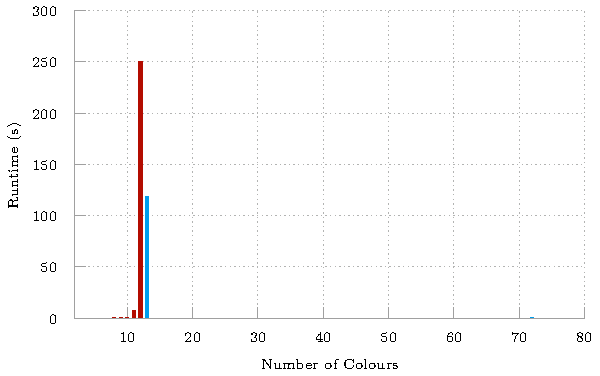
\includegraphics{gen-graph-gcol-decisions.pdf}
    }
\end{frame}

\begin{frame}{Parallel In Theory}
    \only<1>{
        \begin{itemize}
            \item \emph{Speedup} is sequential runtime divided by parallel runtime.
                \begin{itemize}
                    \item Ideally, over a good sequential algorithm, not a parallel algorithm run with one
                        thread. This is sometimes called \emph{absolute} speedup.
                    \item This may not be practical if using special hardware.
                \end{itemize}

            \item A \emph{linear} speedup is a speedup of $n$ using $n$ processors.
                \begin{itemize}
                    \item This is not a realistic expectation on modern hardware. Of particular
                        concern for CP is that more cores does not mean more memory bandwidth.
                \end{itemize}
        \end{itemize}
    }

    \only<2>{
        \begin{itemize}
            \item \emph{Balance} is whether every compute unit is kept busy doing useful work.

            \item A \emph{regular} problem is one which can easily be split into equally sized units of
                work. Irregular problems are hard to balance.

            \item Often only a small number of the decision problems are ``really hard'', so we get poor
                balance.
        \end{itemize}
    }

    \only<3>{
        \begin{itemize}
            \item Most parallel algorithms contain a ``sequential'' part which cannot be parallelised,
                and a ``parallel'' part.

            \item \emph{Amdahl's law} says that if the sequential portion is fixed and we divide the
                parallel portion perfectly among $n$ processors, and if $k$ is the fraction of the
                work we cannot parallelise, then \[
                    \mathit{best~speedup} = \frac{1}{k + \frac{1}{n}\left(1 - k\right)}
                \]

            \item For CP algorithms, things get much more complicated, so it is important to understand
                where the formula comes from (using primary school maths), rather than memorising it.

            \item \emph{Gustafson's law} deals with using more processors to tackle larger problems.
        \end{itemize}
    }

    \only<4>{
        \begin{itemize}
            \item We need a large parallelisable portion of the algorithm, \emph{and} good work
                balance, or we don't get much of an improvement.
        \end{itemize}
    }
\end{frame}

\begin{frame}{Parallel Consistency?}

    \only<1> {
        \begin{itemize}
            \item Partition the variables between processors.
            \item Run AC3 independently on each processor, but when deleting a value, also send a
                message to other processors telling them to re-add the relevant variables to their
                stack.
            \item But maybe only a few variables are involved, and we spend all our time
                bouncing around between a small number of processors\ldots
            \item And what about slow-running global constraints?
        \end{itemize}
    }

    \only<2> {
        \begin{columns}[T]
            \column{.5\textwidth}
            \centering
\includegraphics[keepaspectratio=true,scale=0.12]{disac4-paper.png}

            \column{.5\textwidth}
            \centering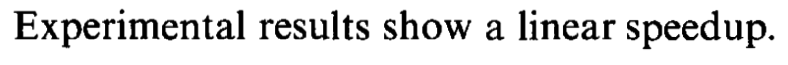
\includegraphics[keepaspectratio=true,scale=0.12]{disac4-linear.png}
            \vspace{0.5em}
            \centering
\includegraphics[keepaspectratio=true,scale=0.12]{disac4-massive.png}
        \end{columns}

        \vspace{3em}

        \begin{columns}[T]
            \column{.5\textwidth}
            \centering
\includegraphics[keepaspectratio=true,scale=0.12]{parallel-consistency-paper.png}

            \column{.5\textwidth}
            \centering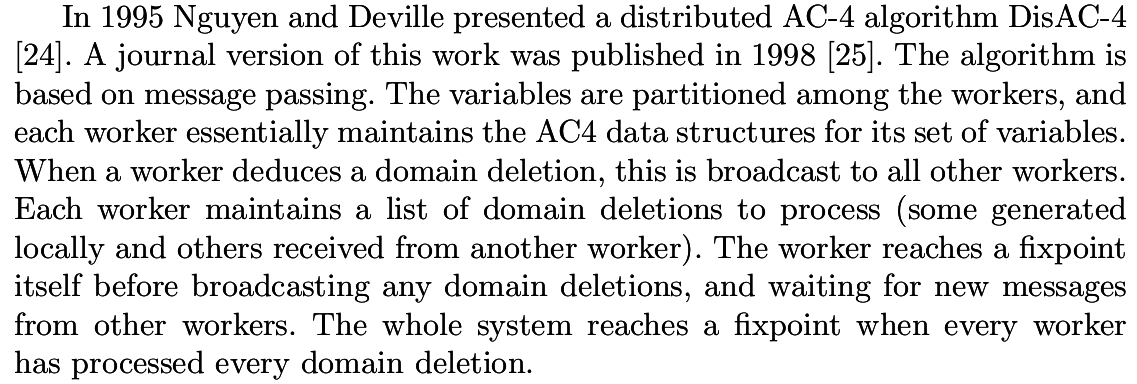
\includegraphics[keepaspectratio=true,scale=0.12]{parallel-consistency-method.png}
            \vspace{1em}
            \centering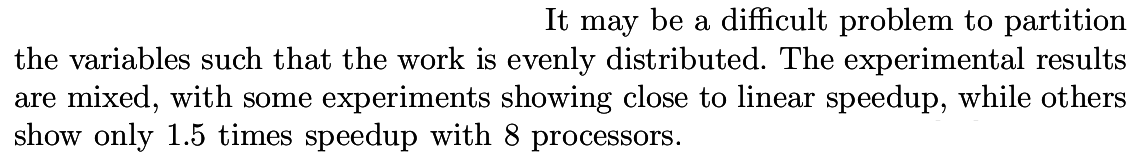
\includegraphics[keepaspectratio=true,scale=0.12]{parallel-consistency-results.png}

        \end{columns}
    }

    \only<3> {
        \begin{center}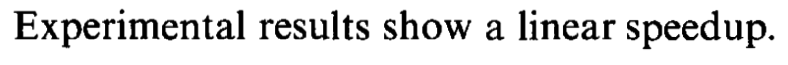
\includegraphics[keepaspectratio=true,scale=0.25]{disac4-linear.png}\end{center}

        \vspace{2em}

        \begin{center}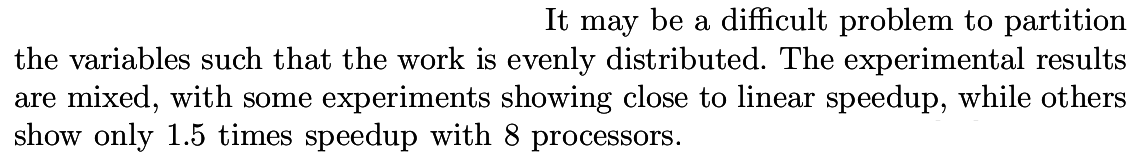
\includegraphics[keepaspectratio=true,scale=0.25]{parallel-consistency-results.png}\end{center}
    }

    \only<4>{
        \centering
\includegraphics[keepaspectratio=true,scale=0.25]{disac4-massive.png}
    }

    \only<5>{
        \centering
\includegraphics[keepaspectratio=true,scale=0.1]{acpc-paper.png}

        \vspace{2em}

        \centering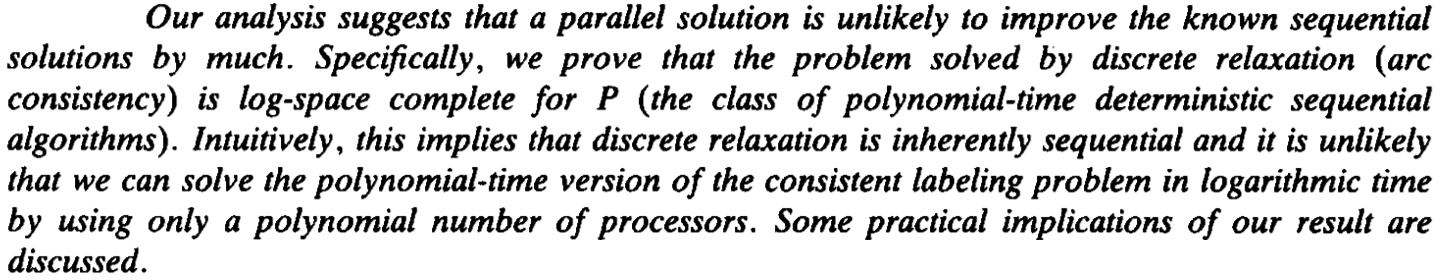
\includegraphics[keepaspectratio=true,scale=0.1]{acpc-abstract.png}

        \vspace{2em}

        \centering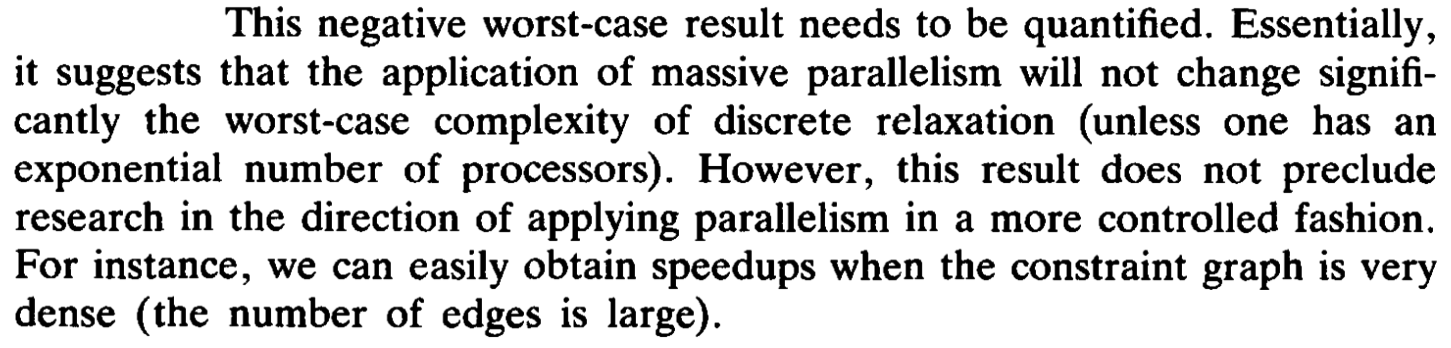
\includegraphics[keepaspectratio=true,scale=0.1]{acpc-practical.png}

        \vspace{0em}
    }

    \only<6>{
        \centering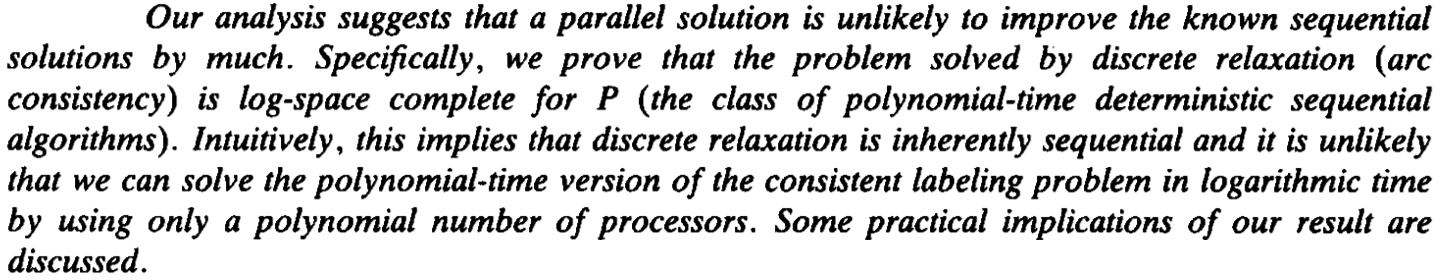
\includegraphics[keepaspectratio=true,scale=0.2]{acpc-abstract.png}

        \vspace{0em}
    }

    \only<7>{
        \centering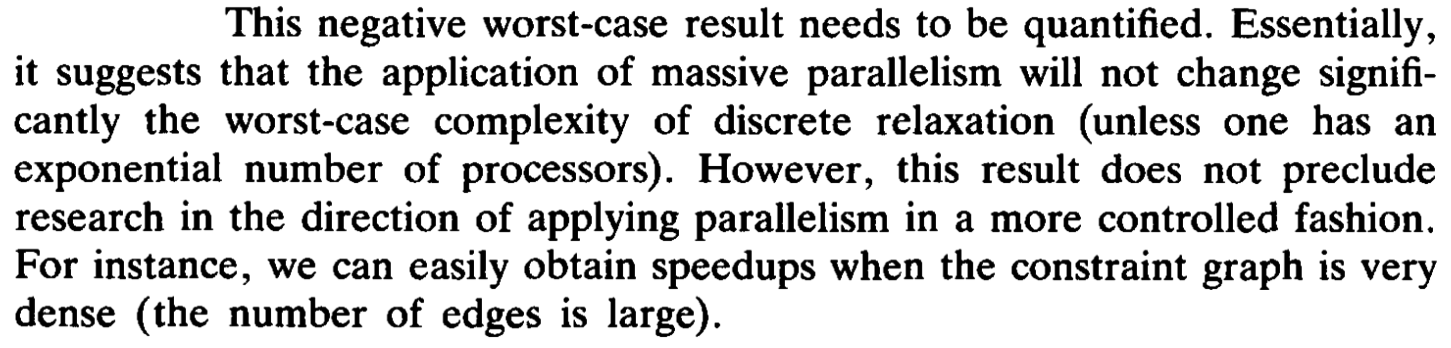
\includegraphics[keepaspectratio=true,scale=0.2]{acpc-practical.png}

        \vspace{0em}
    }

    \only<8> {
        \centering
\includegraphics[keepaspectratio=true,scale=0.4]{acpc-poly.png}

        \vspace{0em}
    }
\end{frame}

\begin{frame}{Bitsets and Bit Parallelism}
    \only<1>{
        \begin{itemize}
            \item Domains are sometimes small and compact.

            \item If domains have no more than 64 values, we can store them in (long unsigned) integers.
                We have one bit per value. $0$ means ``not in the set'' and $1$ means ``in the set''.

            \item We can use arrays of integers for larger domains. (And we can go up to 512 bit
                integers on some Intel CPUs.)
        \end{itemize}
    }

    \only<2>{
        \begin{itemize}
            \item This is hardware-friendly: the entire model might fit in cache.

            \item Setting a domain to take exactly one value: \[
                    d \gets 1 \ll v
                \]

            \item Testing whether or not a value is present in a domain: \[
                    d~\&~(1 \ll v) \ne 0
                \]

            \item Turning a single bit off: \[
                    d \gets d~\&~\text{\textasciitilde}(1 \ll v)
                \]

            \item There are dedicated hardware instructions for all of these in recent CPUs. We can
                also count the number of set bits (how many values are left in our domain?), and
                find the first set bit (pick a value from the domain) in hardware.
        \end{itemize}
    }

    \only<3>{
        \begin{itemize}
            \item Some constraints are similarly bitset friendly.

            \item Table constraints (a list of all ``allowed pairs'') can be represented as
                a ``compatibility'' bitset for each value in each variable's domain. Now
                forward checking is just a bitwise ``and'' operation.
                \begin{itemize}
                    \item Uses a lot of memory, but if our model is reasonably small and dense
                        that's fine.
                \end{itemize}

            \item Less than, greater than, and certain arithmetic constraints work nicely with
                bitsets.
                \begin{itemize}
                    \item Fun exercise: figure this out.
                \end{itemize}

            \item Some constraints are probably not bitset friendly.
        \end{itemize}
    }
\end{frame}

\begin{frame}{Fixed Parallel Tree Search}
    \begin{center}
        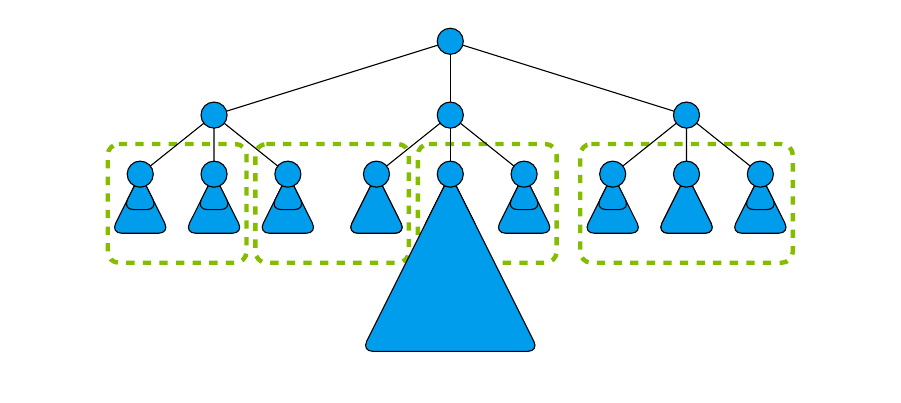
\begin{tikzpicture}[scale=0.75]%{{{
        \coordinate (R);

        \coordinate (N) at (R);

        \coordinate (N1) at ($(N) + (-4, -1.25)$);
        \coordinate (N2) at ($(N) + ( 0, -1.25)$);
        \coordinate (N3) at ($(N) + ( 4, -1.25)$);

        \foreach \na in {1, ..., 3}{
            \coordinate (N\na 1) at ($(N\na) + (-1.25, -1)$);
            \coordinate (N\na 2) at ($(N\na) + ( 0,    -1)$);
            \coordinate (N\na 3) at ($(N\na) + ( 1.25, -1)$);

            \foreach \nb in {1, ..., 3}{
                \coordinate (N\na\nb t1) at ($(N\na\nb) + (-0.5, -1)$);
                \coordinate (N\na\nb t2) at ($(N\na\nb) + ( 0.5, -1)$);

                \coordinate (N\na\nb s1) at ($(N\na\nb) + (-0.3, -0.6)$);
                \coordinate (N\na\nb s2) at ($(N\na\nb) + ( 0.3, -0.6)$);

                \coordinate (N\na\nb h1) at ($(N\na\nb) + (-1.5, -3)$);
                \coordinate (N\na\nb h2) at ($(N\na\nb) + ( 1.5, -3)$);
            }
        }

        \tikzstyle{p} = [draw, rounded corners, dashed, color=uofglawn, ultra thick];
        \draw <2-3> [p] ($(N11) + (-0.55, 0.51)$) -- ($(N12) + (0.55, 0.51)$) -- ($(N12) + (0.55, -1.5)$) -- ($(N11) + (-0.55, -1.5)$) -- cycle;
        \draw <2-3> [p] ($(N13) + (-0.55, 0.51)$) -- ($(N21) + (0.55, 0.51)$) -- ($(N21) + (0.55, -1.5)$) -- ($(N13) + (-0.55, -1.5)$) -- cycle;
        \draw <2-3> [p] ($(N22) + (-0.55, 0.51)$) -- ($(N23) + (0.55, 0.51)$) -- ($(N23) + (0.55, -1.5)$) -- ($(N22) + (-0.55, -1.5)$) -- cycle;
        \draw <2-3> [p] ($(N31) + (-0.55, 0.51)$) -- ($(N33) + (0.55, 0.51)$) -- ($(N33) + (0.55, -1.5)$) -- ($(N31) + (-0.55, -1.5)$) -- cycle;

        \foreach \na in {1, ..., 3}{
            \draw (N) -- (N\na);
            \foreach \nb in {1, ..., 3}{
                \draw (N\na) -- (N\na\nb);
            }
        }

        \tikzstyle{t} = [draw, fill, fill=uofgcobalt, rounded corners];
        \foreach \na in {1, ..., 3}{
            \foreach \nb in {1, ..., 3}{
                \draw <1-2> [t] (N\na\nb) -- (N\na\nb t1) -- (N\na\nb t2) -- cycle;
            }
        }

        \draw <3> [t] (N11) -- (N11s1) -- (N11s2) -- cycle;
        \draw <3> [t] (N12) -- (N12s1) -- (N12s2) -- cycle;
        \draw <3> [t] (N13) -- (N13s1) -- (N13s2) -- cycle;

        \draw <3> [t] (N21) -- (N21t1) -- (N21t2) -- cycle;
        \draw <3> [t] (N22) -- (N22h1) -- (N22h2) -- cycle;
        \draw <3> [t] (N23) -- (N23s1) -- (N23s2) -- cycle;

        \draw <3> [t] (N31) -- (N31s1) -- (N31s2) -- cycle;
        \draw <3> [t] (N32) -- (N32t1) -- (N32t2) -- cycle;
        \draw <3> [t] (N33) -- (N33s1) -- (N33s2) -- cycle;

        \tikzstyle{c} = [draw, circle, fill, fill=uofgcobalt];
        \node [c] at (N) { };

        \foreach \na in {1, ..., 3}{
            \node [c] at (N\na) { };

            \foreach \nb in {1, ..., 3}{
                \node [c] at (N\na\nb) { };
            }
        }

        \node at (-7, -5.5) { }; \node at (7, -5.5) { };
    \end{tikzpicture}%}}}
    \end{center}
\end{frame}

\begin{frame}{Embarrassingly Parallel Search}
    \only<1>{%
        \begin{itemize}
            \item If we create $n$ subproblems, chances are we'll get poor balance.
            \item We can't tell beforehand where the really hard subproblems will be.
            \item What if we create \emph{lots} of subproblems, and distribute them dynamically?
        \end{itemize}
    }\only<2>{%
        \centering
        
\includegraphics[keepaspectratio=true,scale=0.15]{eps-paper.png}
    }\only<3>{%
        \centering
        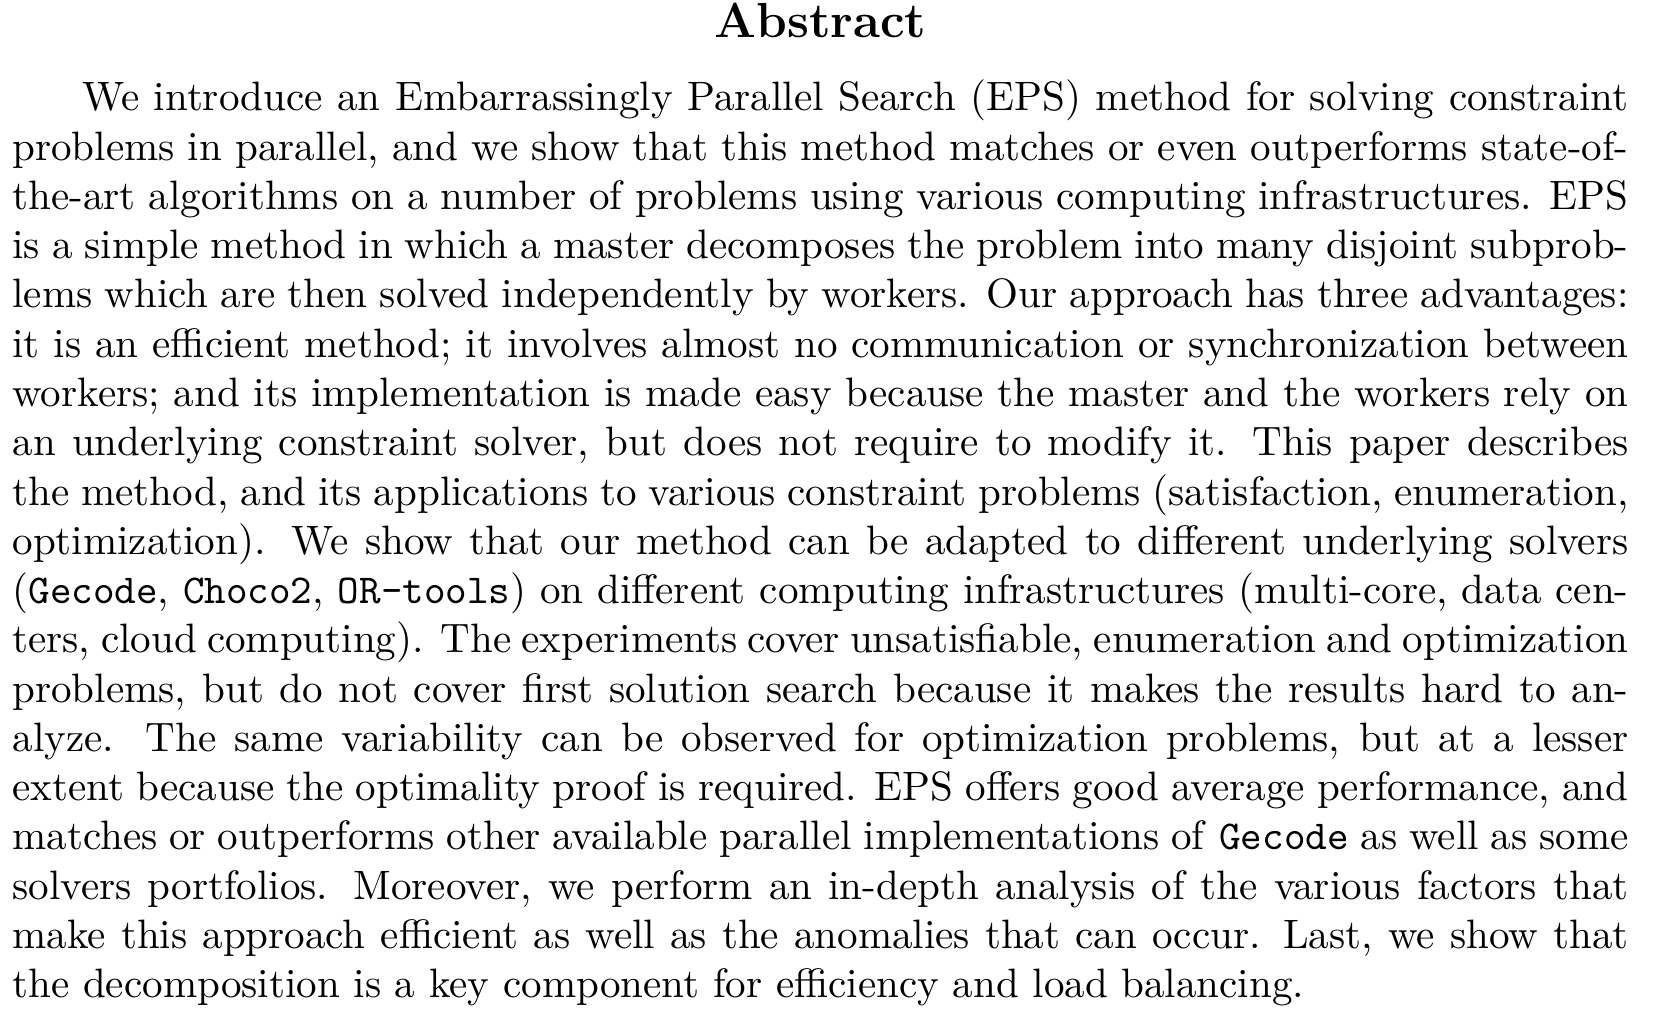
\includegraphics[keepaspectratio=true,scale=0.15]{eps-abstract.png}
    }\only<4>{%
        \centering
        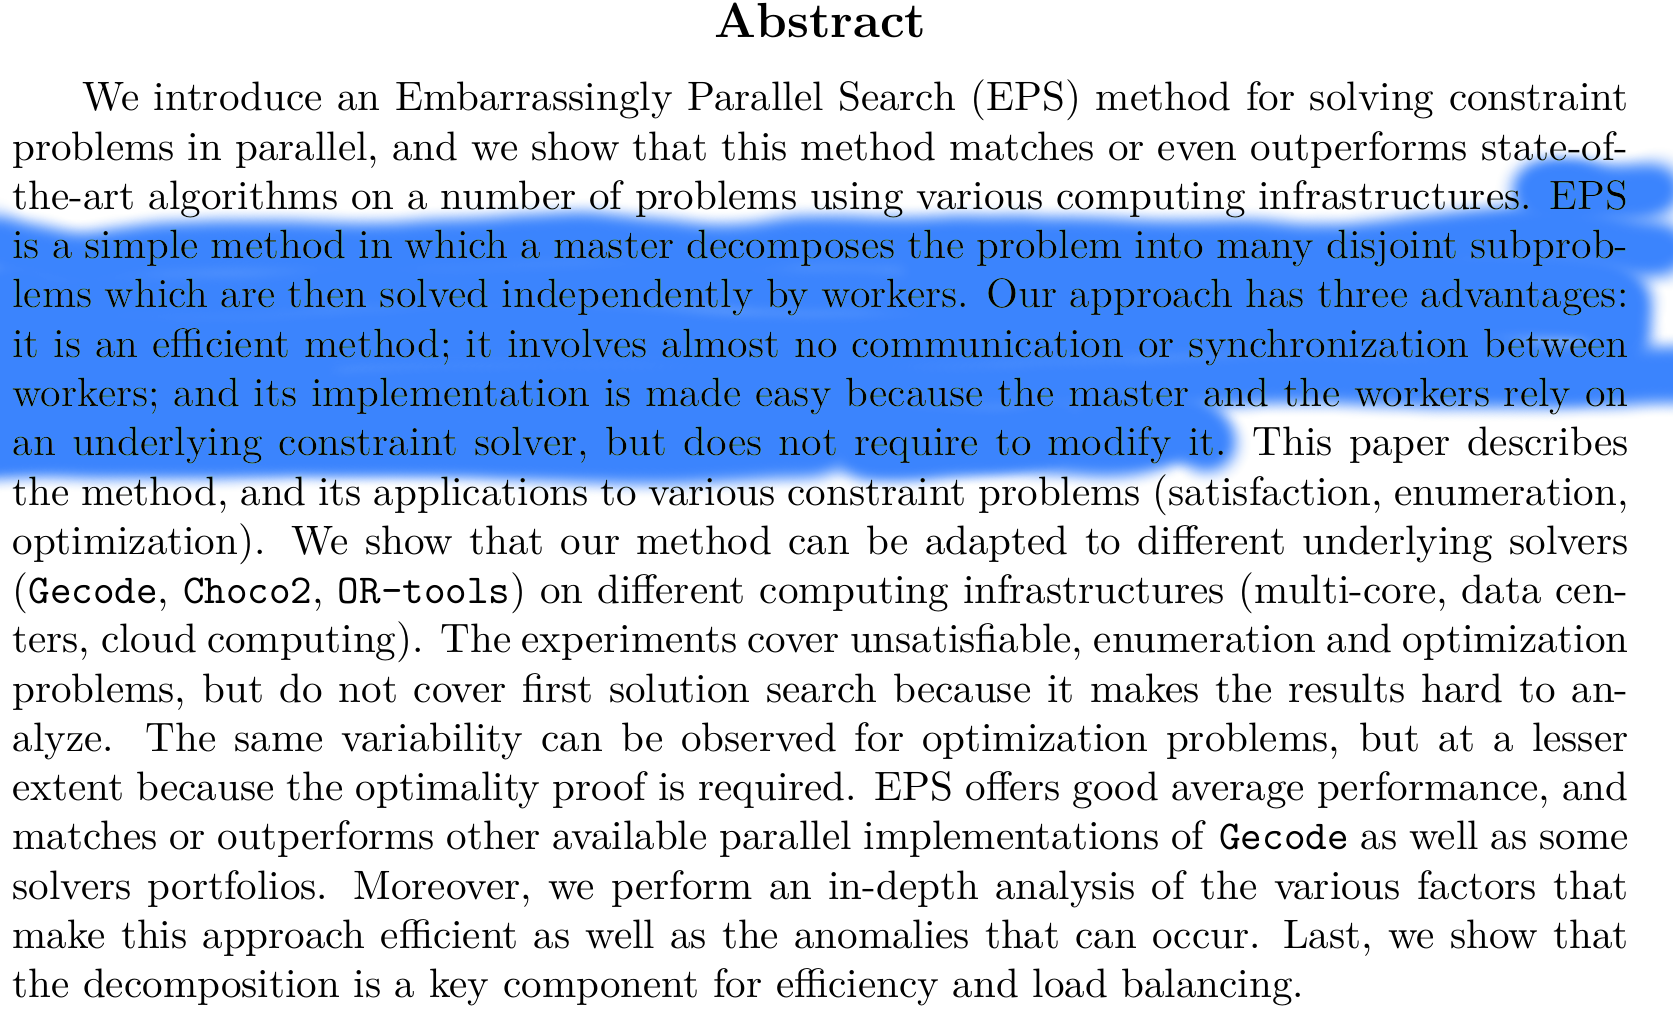
\includegraphics[keepaspectratio=true,scale=0.15]{eps-abstract-idea.png}
    }\only<5>{%
        \centering
        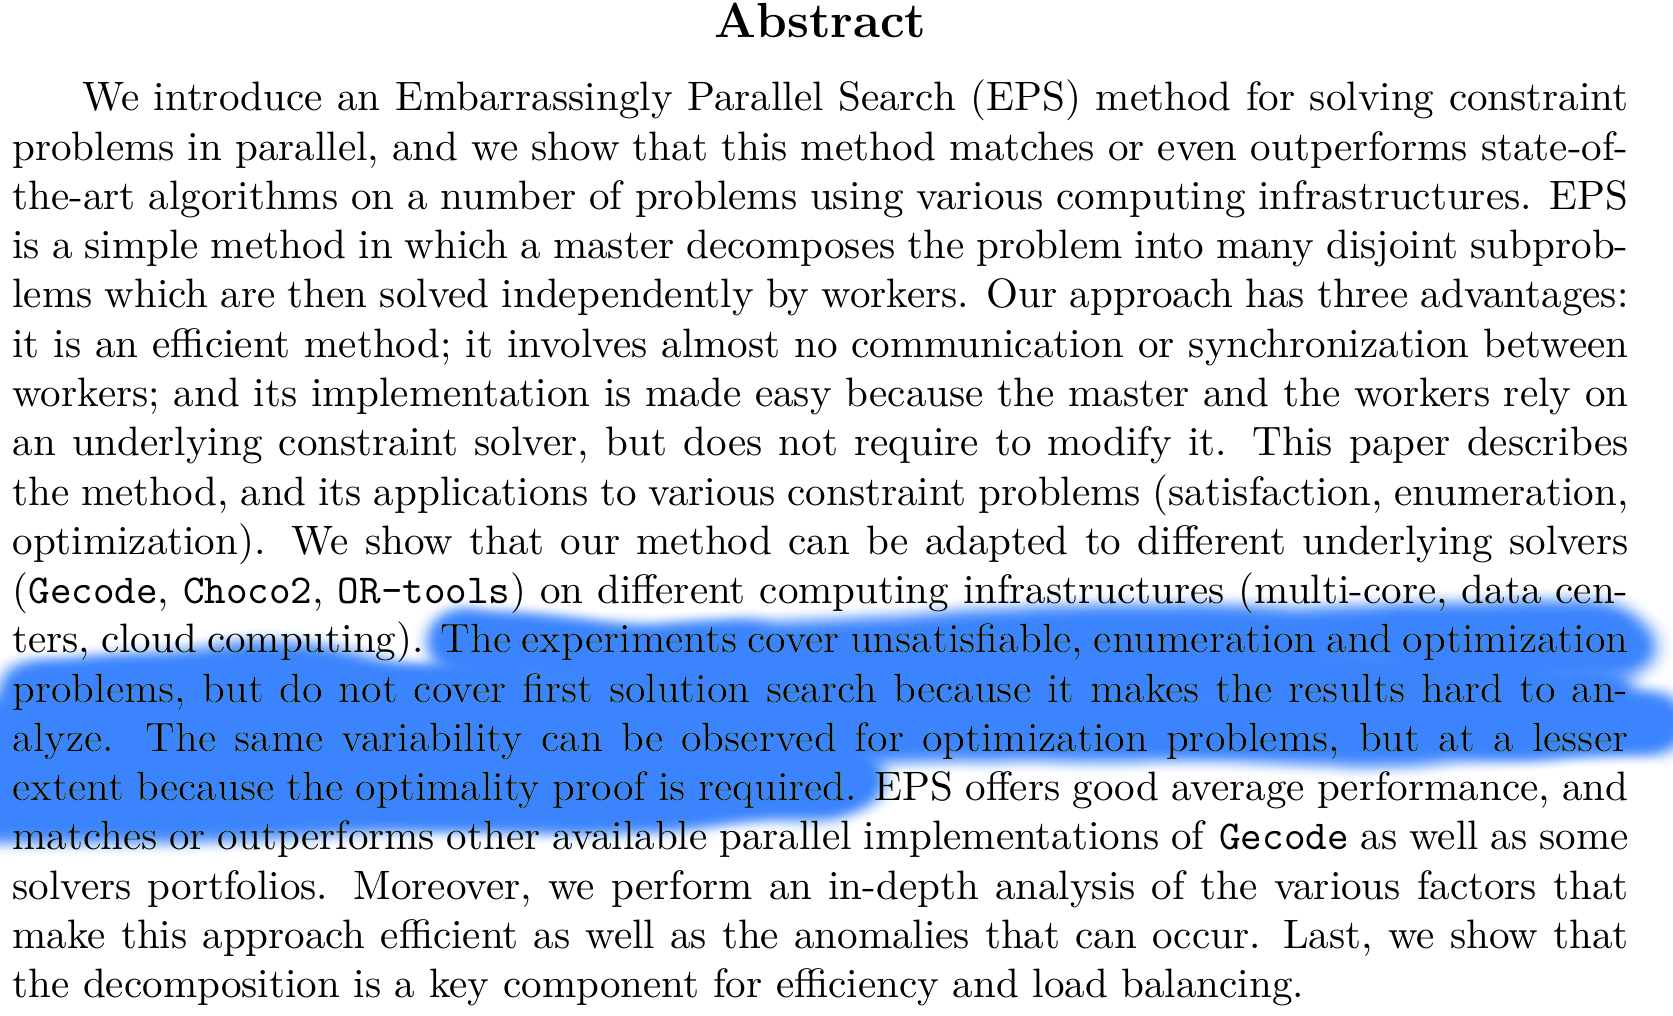
\includegraphics[keepaspectratio=true,scale=0.15]{eps-abstract-decision.png}
    }
\end{frame}

\begin{frame}{Random Work Stealing}
    \only<1> {
        \begin{itemize}
            \item What if we split work entirely dynamically?
            \item Whenever a worker is idle, have it steal a subproblem from another randomly
                selected worker.
        \end{itemize}
    }\only<2>{
        \begin{center}
            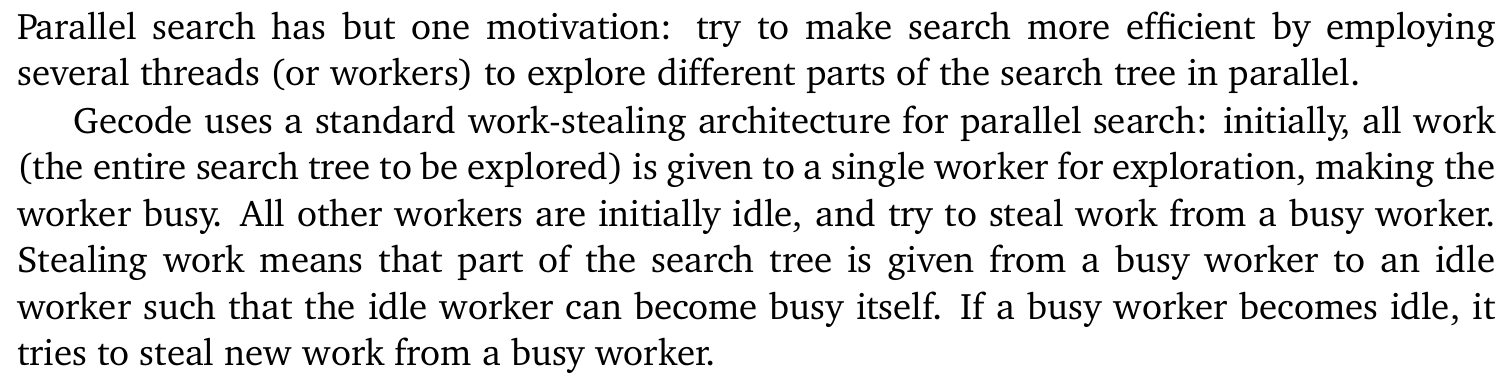
\includegraphics[keepaspectratio=true,scale=0.18]{gecode-parallel.png}
        \end{center}
    }\only<3>{
        \begin{center}
            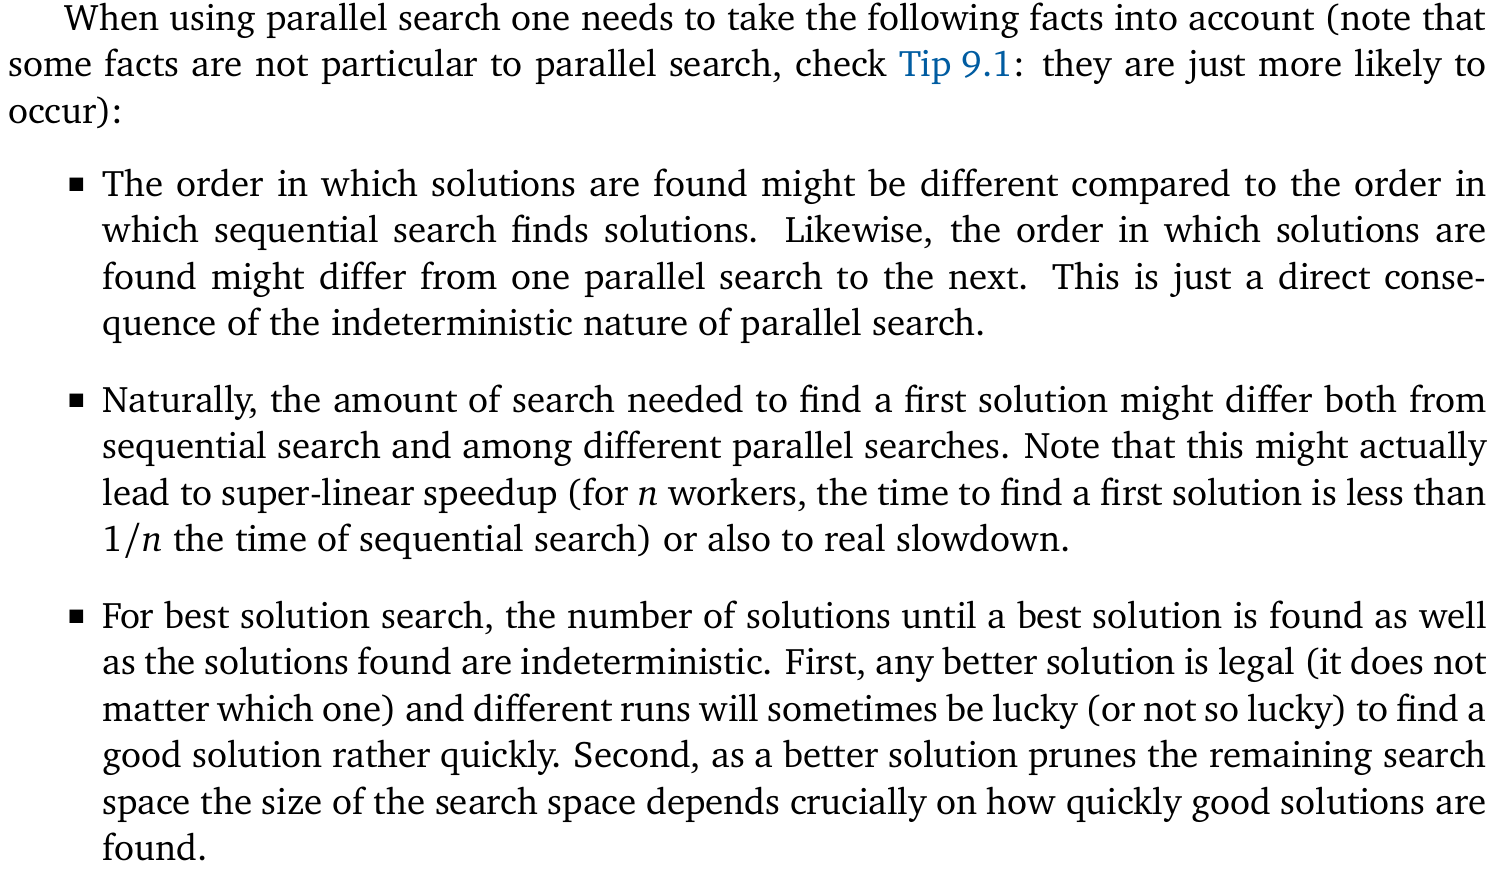
\includegraphics[keepaspectratio=true,scale=0.18]{gecode-facts1.png}
        \end{center}
    }\only<4>{
        \begin{center}
            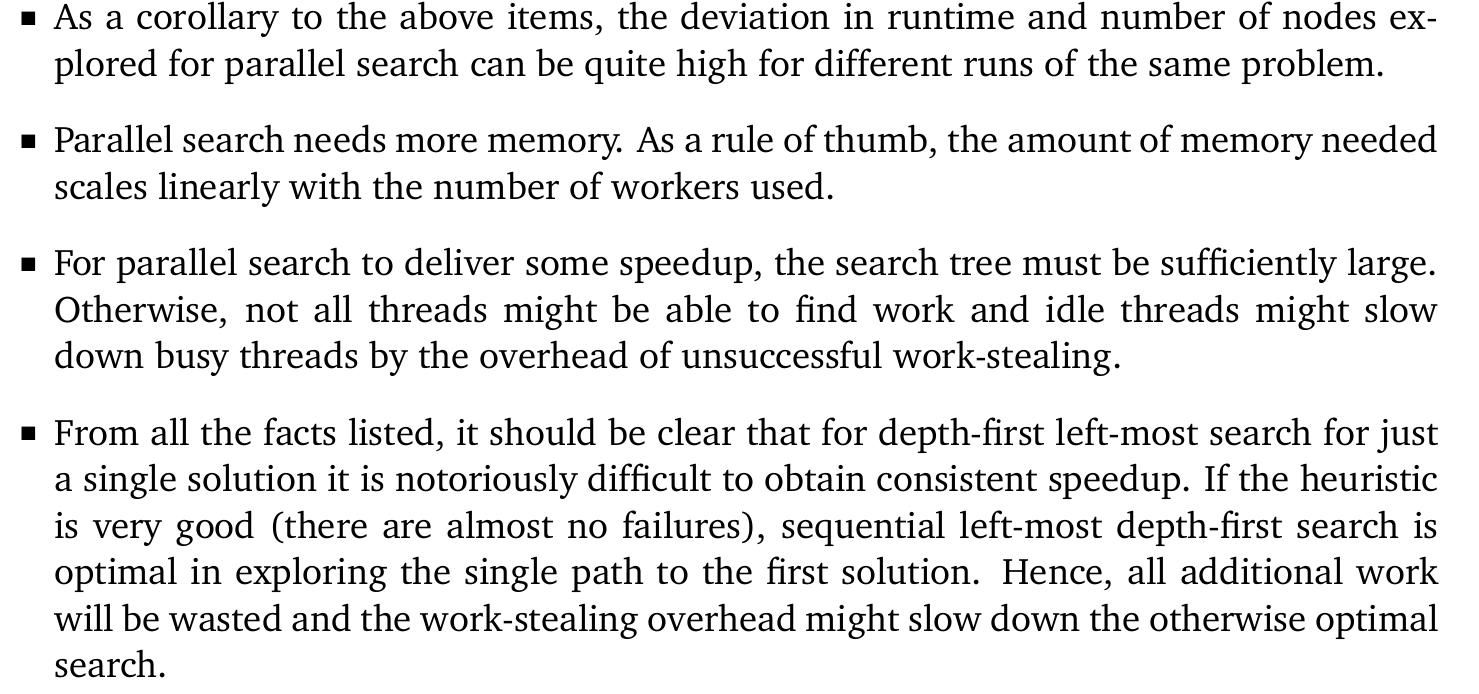
\includegraphics[keepaspectratio=true,scale=0.18]{gecode-facts2.png}
        \end{center}
    }\only<5>{
        \begin{center}
            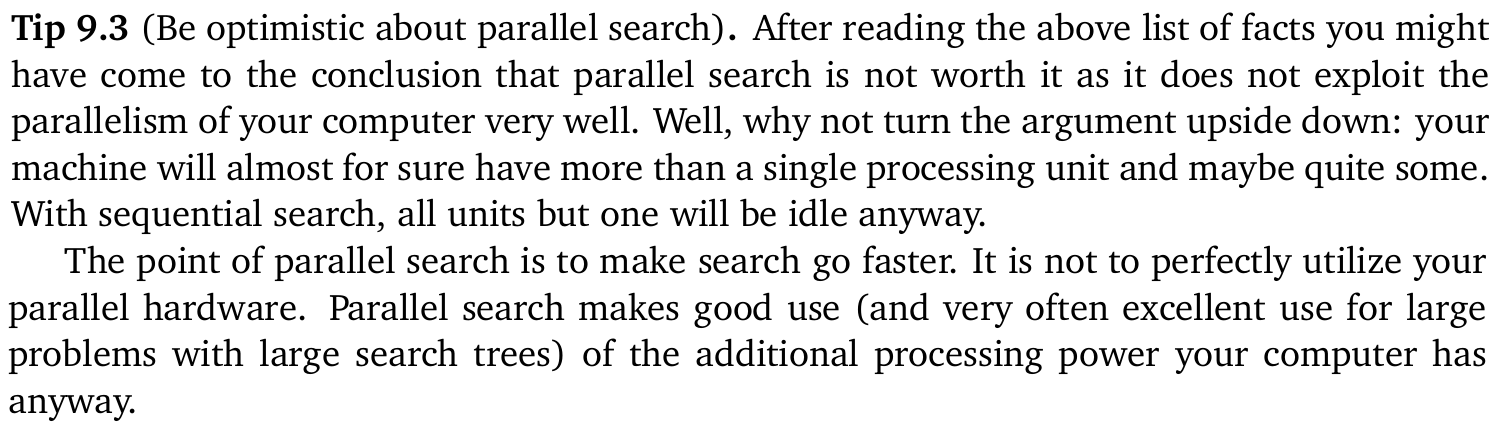
\includegraphics[keepaspectratio=true,scale=0.18]{gecode-optimistic.png}
        \end{center}
    }\only<6>{
        \lstinputlisting[basicstyle=\tiny\ttfamily, keywordstyle=\color{uofgcobalt}]{code/colOpt-g80-p32-runtimes.txt}
    }\only<7>{
        \lstinputlisting[basicstyle=\tiny\ttfamily, keywordstyle=\color{uofgcobalt}]{code/colDec-g80-12-p32-runtimes.txt}
    }\only<8>{
        \lstinputlisting[basicstyle=\tiny\ttfamily, keywordstyle=\color{uofgcobalt}]{code/colDec-g80-13-p32-runtimes.txt}
    }
\end{frame}

\begin{frame}{Speedups from Parallel Tree Search}

    \only<1>{
        \begin{itemize}
            \item If a decision problem is satisfiable, or for an optimisation problem, our speedups
                could be arbitrary: one worker might find a feasible or strong solution very quickly. In
                particular, \emph{superlinear} speedups are possible, as are no speedups at all.

            \item For an unsatisfiable decision problem, or for an enumeration problem, our speedups
                can be at best linear (assuming we do not change the search tree): we \emph{are}
                dividing up a fixed amount of work.

            \item If we do not communicate bounds, or if we do not preserve sequential ordering, we
                could get an \emph{absolute slowdown}.
        \end{itemize}
    }
\end{frame}

\begin{frame}{Work Splitting Affects Search}

    \only<1-3>{
        \begin{center}
            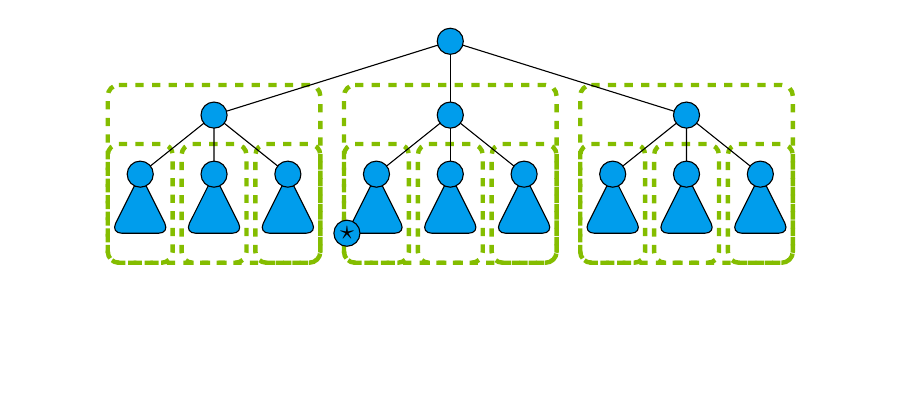
\begin{tikzpicture}[scale=0.75]%{{{
            \coordinate (R);

            \coordinate (N) at (R);

            \coordinate (N1) at ($(N) + (-4, -1.25)$);
            \coordinate (N2) at ($(N) + ( 0, -1.25)$);
            \coordinate (N3) at ($(N) + ( 4, -1.25)$);

            \foreach \na in {1, ..., 3}{
                \coordinate (N\na 1) at ($(N\na) + (-1.25, -1)$);
                \coordinate (N\na 2) at ($(N\na) + ( 0,    -1)$);
                \coordinate (N\na 3) at ($(N\na) + ( 1.25, -1)$);

                \foreach \nb in {1, ..., 3}{
                    \coordinate (N\na\nb t1) at ($(N\na\nb) + (-0.5, -1)$);
                    \coordinate (N\na\nb t2) at ($(N\na\nb) + ( 0.5, -1)$);

                    \coordinate (N\na\nb s1) at ($(N\na\nb) + (-0.3, -0.6)$);
                    \coordinate (N\na\nb s2) at ($(N\na\nb) + ( 0.3, -0.6)$);

                    \coordinate (N\na\nb h1) at ($(N\na\nb) + (-1.5, -3)$);
                    \coordinate (N\na\nb h2) at ($(N\na\nb) + ( 1.5, -3)$);
                }
            }

            \tikzstyle{p} = [draw, rounded corners, dashed, color=uofglawn, ultra thick];
            \foreach \na in {1, ..., 3}{
                \foreach \nb in {1, ..., 3}{
                    \draw <1-2> [p] ($(N\na\nb) + (-0.55, 0.51)$) -- ($(N\na\nb) + (0.55, 0.51)$) --
                        ($(N\na\nb) + (0.55, -1.5)$) -- ($(N\na\nb) + (-0.55, -1.5)$) -- cycle;
                }

                \draw <3> [p] ($(N\na 1) + (-0.55, 1.51)$) -- ($(N\na 3) + (0.55, 1.51)$) --
                    ($(N\na 3) + (0.55, -1.5)$) -- ($(N\na 1) + (-0.55, -1.5)$) -- cycle;
            }

            \foreach \na in {1, ..., 3}{
                \draw (N) -- (N\na);
                \foreach \nb in {1, ..., 3}{
                    \draw (N\na) -- (N\na\nb);
                }
            }

            \tikzstyle{t} = [draw, fill, fill=uofgcobalt, rounded corners];
            \foreach \na in {1, ..., 3}{
                \foreach \nb in {1, ..., 3}{
                    \draw [t] (N\na\nb) -- (N\na\nb t1) -- (N\na\nb t2) -- cycle;
                }
            }

            \tikzstyle{c} = [draw, circle, fill, fill=uofgcobalt];
            \node [c] at (N) { };

            \foreach \na in {1, ..., 3}{
                \node [c] at (N\na) { };

                \foreach \nb in {1, ..., 3}{
                    \node [c] at (N\na\nb) { };
                }
            }

            \node <2-3> [c] at (N21t1) { };
            \node <2-3> at (N21t1) { $\star$ };

            \node at (-7, -5.5) { }; \node at (7, -5.5) { };
        \end{tikzpicture}%}}}
        \end{center}
    }

    \only<4>{
        \begin{itemize}
            \item For satisfiable instances and optimisation problems, where you split the work doesn't just
                affect balance. It also affects the amount of work to do. We just saw an example where
                \emph{better} work balance gave \emph{worse} performance, because it took longer to
                find a solution.

            \item Value-ordering heuristics are most likely to wrong higher up in the tree (there is
                least information available when no or few choices have been made).

            \item Stealing early or splitting high introduces diversity against early heuristic
                choices. Stealing late gives a close-to-sequential ordering.
        \end{itemize}
    }

\end{frame}

\begin{frame}{Parallel Discrepancy Search}
    \only<1>{
        \centering
\includegraphics[keepaspectratio=true,scale=0.4]{parallel-lds-thesis.png}
    }
\end{frame}

\begin{frame}{Confidence-Based Work Stealing}

    \only<1>{
        \centering
\includegraphics[keepaspectratio=true,scale=0.35]{cows-paper.png}
    }

    \only<2>{
        \centering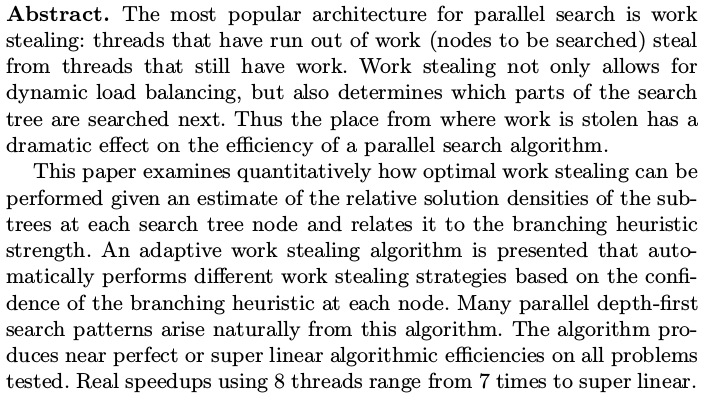
\includegraphics[keepaspectratio=true,scale=0.35]{cows-abstract.png}
    }

    \only<3>{
        \centering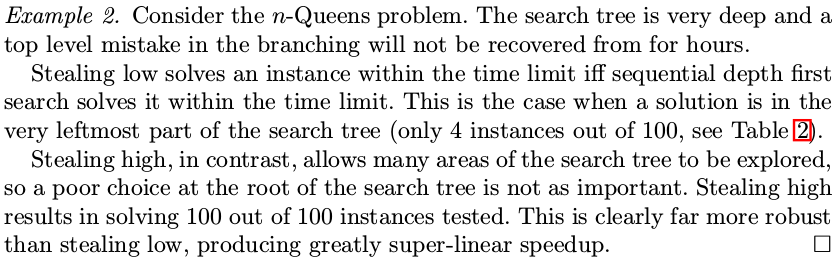
\includegraphics[keepaspectratio=true,scale=0.35]{cows-early.png}
    }

    \only<4>{
        \centering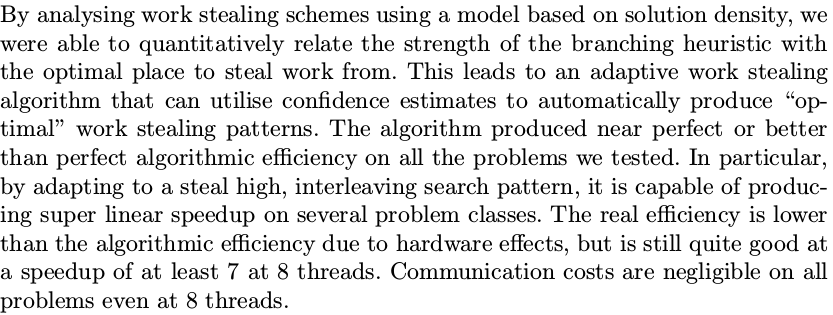
\includegraphics[keepaspectratio=true,scale=0.35]{cows-conclusion.png}
    }

\end{frame}

\begin{frame}{Using Confidence-Based Work Stealing}
    \begin{itemize}
        \item Unfortunately, you can't\ldots
    \end{itemize}
\end{frame}

\begin{frame}{Parallel Portfolios?}
    \only<1>{
    \begin{itemize}
        \item We might have several models, several variable- and value-ordering heuristics,
            tiebreaking, etc.
        \item Just run them all, and pick whichever finishes first?
        \item We can share incumbents and bounds between models.
    \end{itemize}
}\only<2>{
    \centering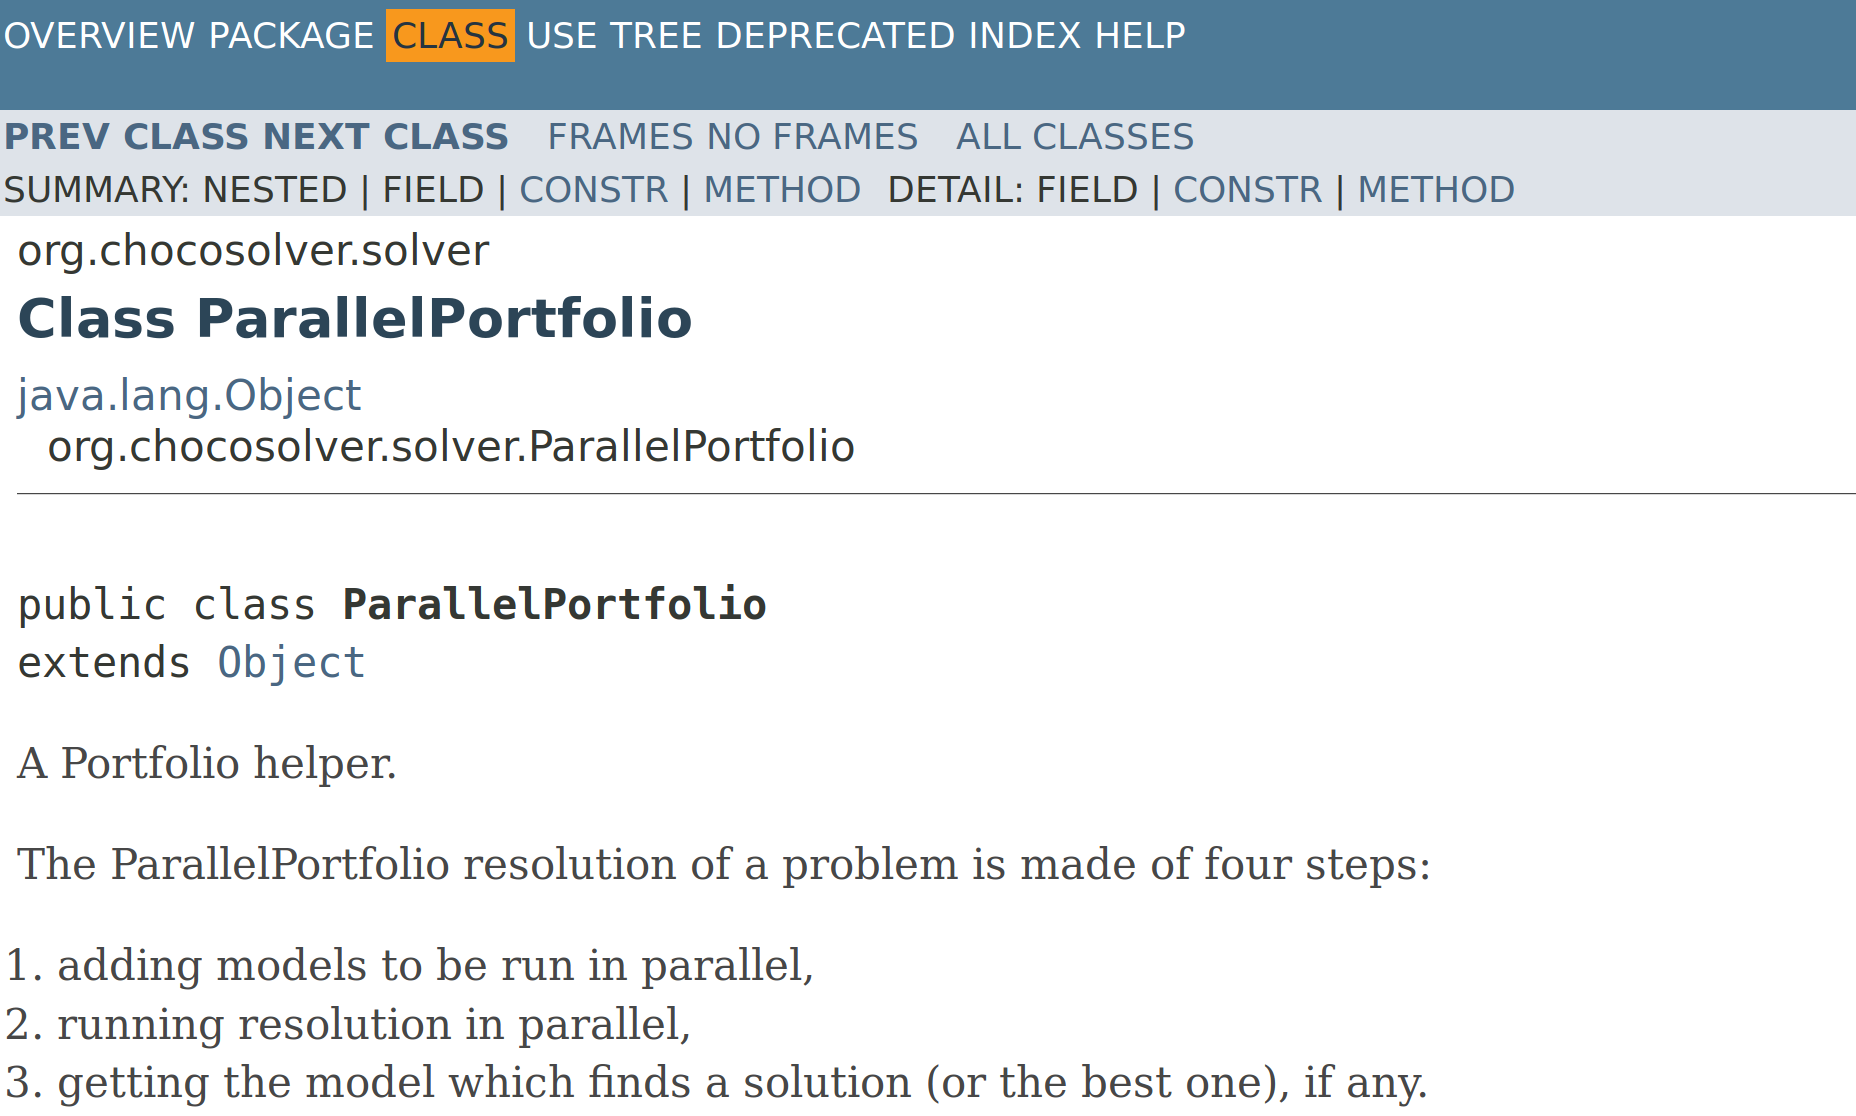
\includegraphics[keepaspectratio=true,scale=0.15]{portfolios-javadoc.png}
}\only<3>{
    \centering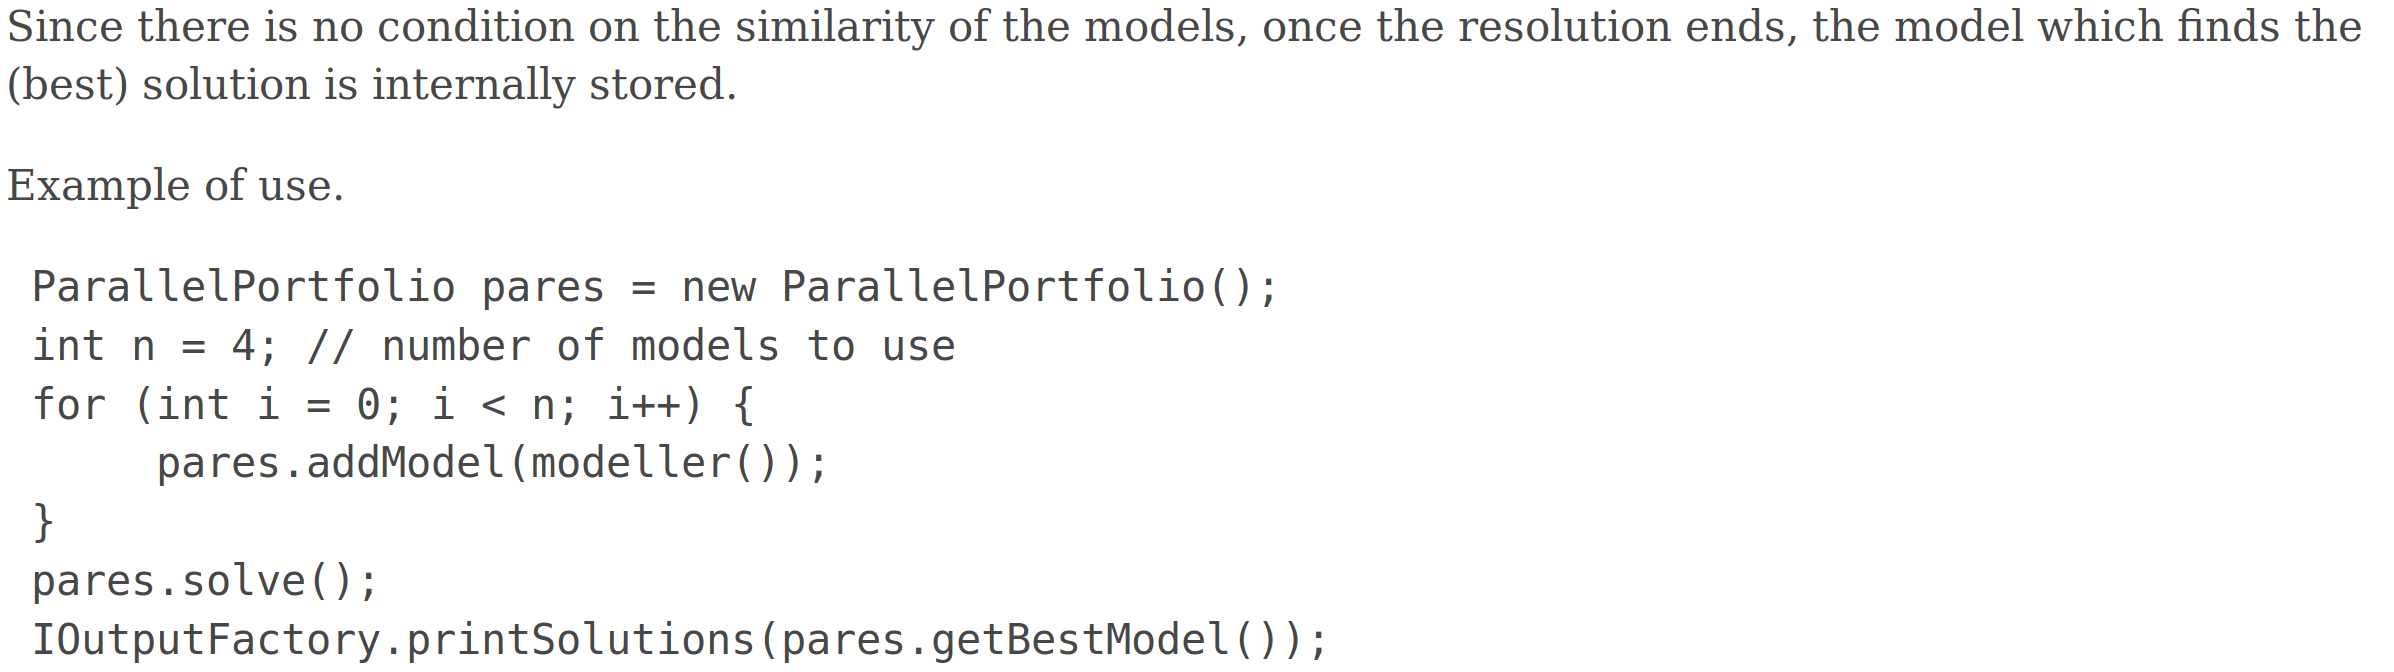
\includegraphics[keepaspectratio=true,scale=0.12]{portfolios-example.png}
}
\end{frame}

\begin{frame}{Parallel Restarts and Random Value-Ordering}
    \only<1>{
        \begin{itemize}
            \item Use random or biased-random search with restarts and nogood recording.
            \item Give each thread its own random seed.
            \item Share nogoods using a barrier on restarts.
        \end{itemize}
    }\only<2>{
        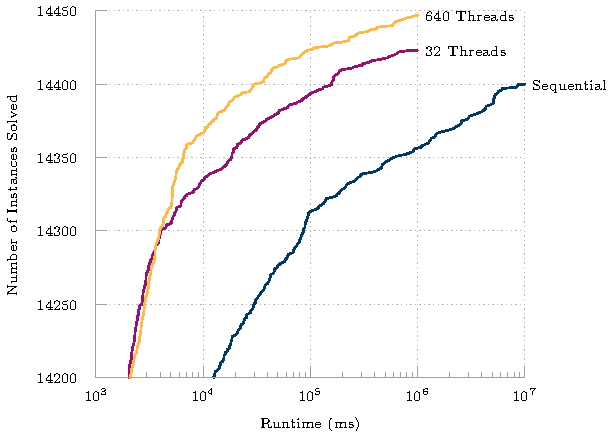
\includegraphics{gen-graph-psbs.pdf}%
    }
\end{frame}

\begin{frame}{This is Not The Exam Question}

    \scriptsize

    A constraint model takes 10 seconds to solve using one processor. Suppose 80\% of that time is
    spent doing propagation. What is the best possible speedup that could be obtained if 4
    processors are used to do parallel propagation, and the rest of the program remains
    unchanged? What about if we had an unlimited number of processors?
    \\[0.5cm]

    What about if we used the four processors for a portfolio of different solvers? \\[0.5cm]

    What is \emph{balance}, and why is it a problem if we try to parallelise a tree-search by
    creating $n$ sub-trees for $n$ processors? Suggest two potential remedies. \\[0.5cm]

    Suppose we are solving a decision problem which has a sequential part taking
    one second to run, and a parallelisable part which takes twenty seconds to run on one
    processor. What is the best possible runtime we might see when using ten processors to
    solve this problem with a parallel tree-search, if the instance is satisfiable? What if
    it is unsatisfiable? \\[0.5cm]

    Design a parallel constraint programming approach that always gives linear speedups.

\end{frame}

\begin{frame}[plain,noframenumbering]
    \begin{tikzpicture}[remember picture, overlay]
        \node at (current page.north west) {
            \begin{tikzpicture}[remember picture, overlay]
                \fill [fill=uofguniversityblue, anchor=north west] (0, 0) rectangle (\paperwidth, -1.7cm);
            \end{tikzpicture}
        };

        \node (logo) [anchor=north east, shift={(-0.3cm,-0.2cm)}] at (current page.north east) {
            
\includegraphics[keepaspectratio=true,scale=0.55]{UoG_keyline.pdf}
        };
    \end{tikzpicture}
\end{frame}

\end{document}

